%%%%%%%%%%%%%%%%%%%%%%%%%%%%%%%%%%%%

For boosted Higgs searches, the invariant mass of the $b\bar b$ system is of interest. The analysis is capable of studying the unnormalized (track) invariant mass of the $b\bar b $ system. The analogues to Fig.~\ref{fig:gbbdistributions} and~\ref{fig:gbbresponse} for the mass are shown in Fig.~\ref{fig:gbbdistributionsm} and~\ref{fig:gbbresponsemass}, respectively. The same fit study as for other observables is presented. The MC distribution of $m_{b\bar b}$ is shown in Fig. \ref{fig:trkmass}. Flavor fraction fits are performed in three bins of $m_{b\bar b} $. The MC prediction and fitted fractions of each flavor is shown in Fig. \ref{fig:trkmass-fitfrac}. 

\begin{figure}[htpb!]
\begin{center}
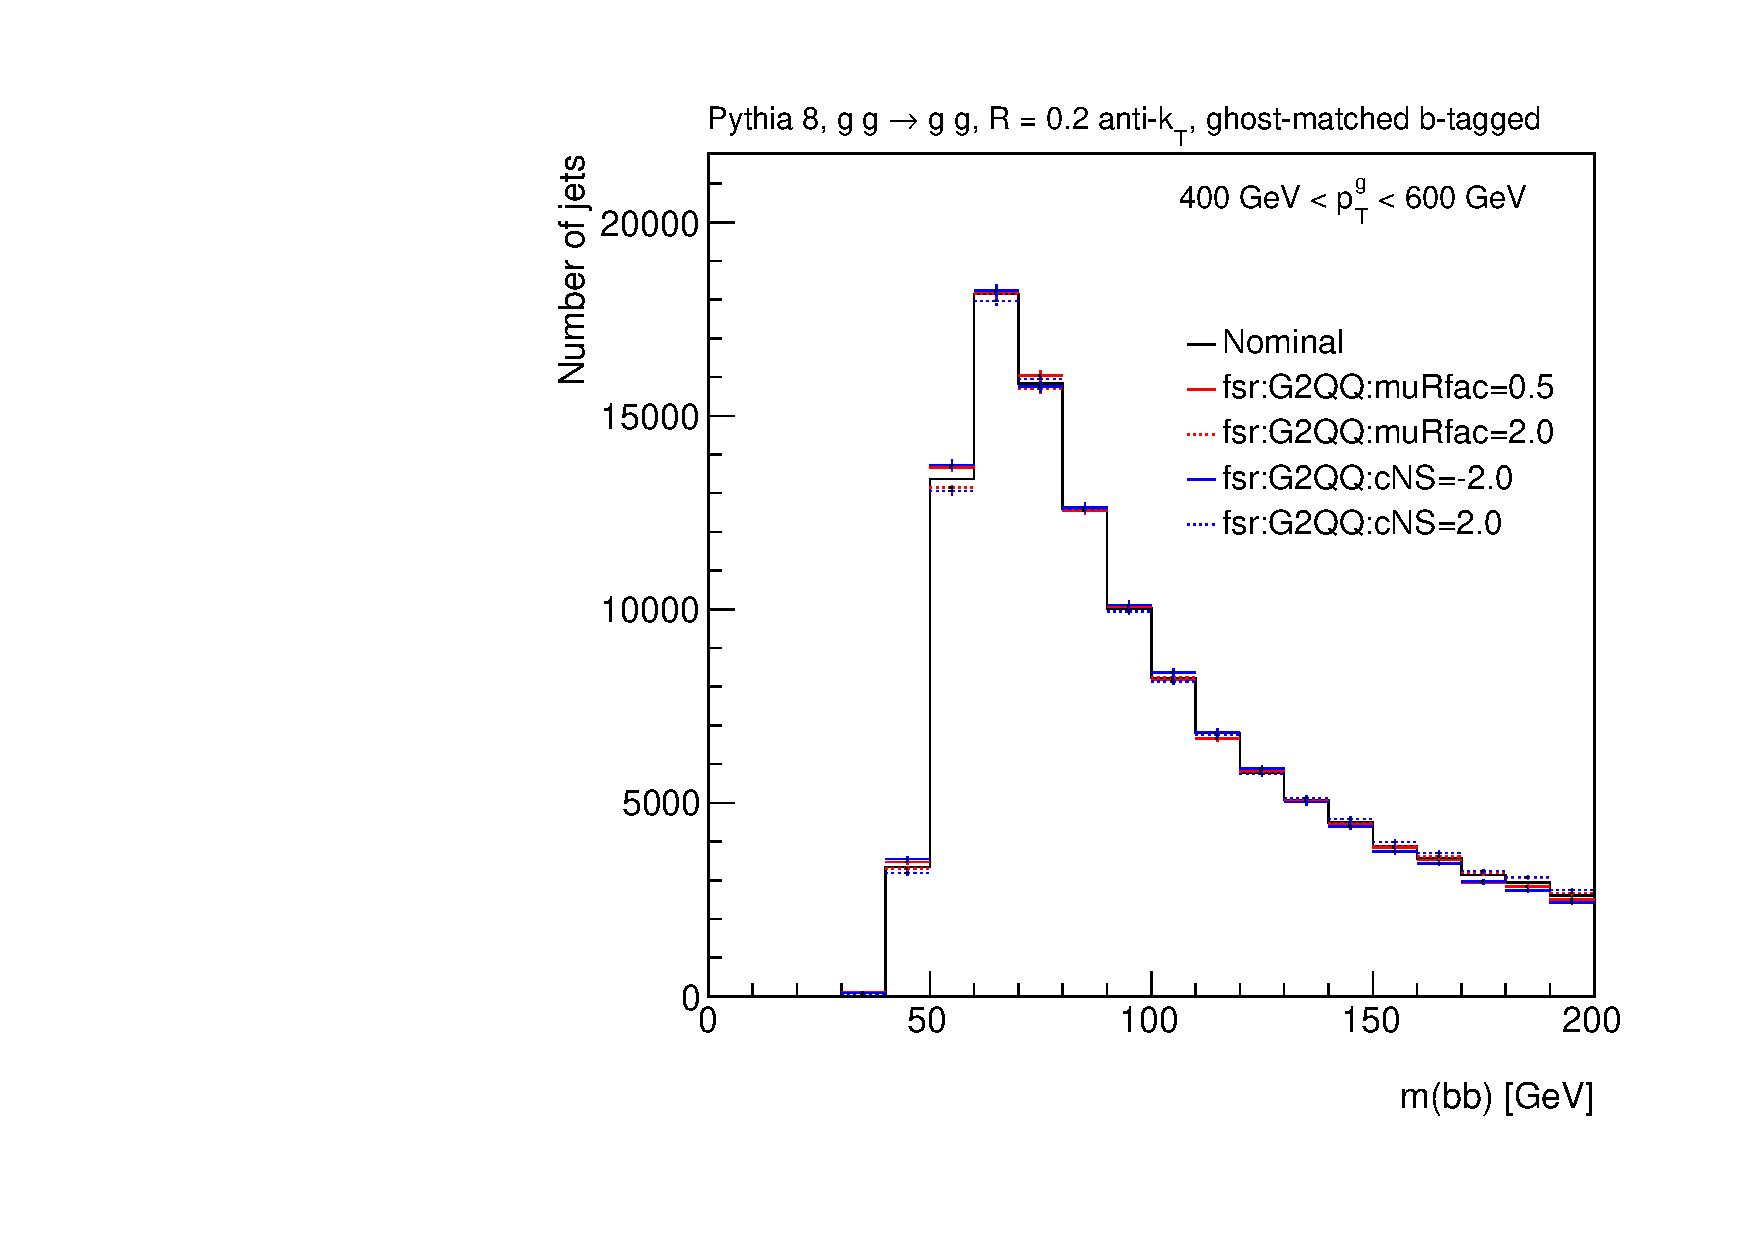
\includegraphics[width=0.33\linewidth]{figures/truth_level/mbb.pdf}
\caption[]{The distribution of $m_{bb}$ in simulation along with a series of variations in the form of the fragmentation described by Pythia~\cite{pythiavariations}.} 
\label{fig:gbbdistributionsm}
\end{center}
\end{figure}

\begin{figure}[htpb!]
\begin{center}
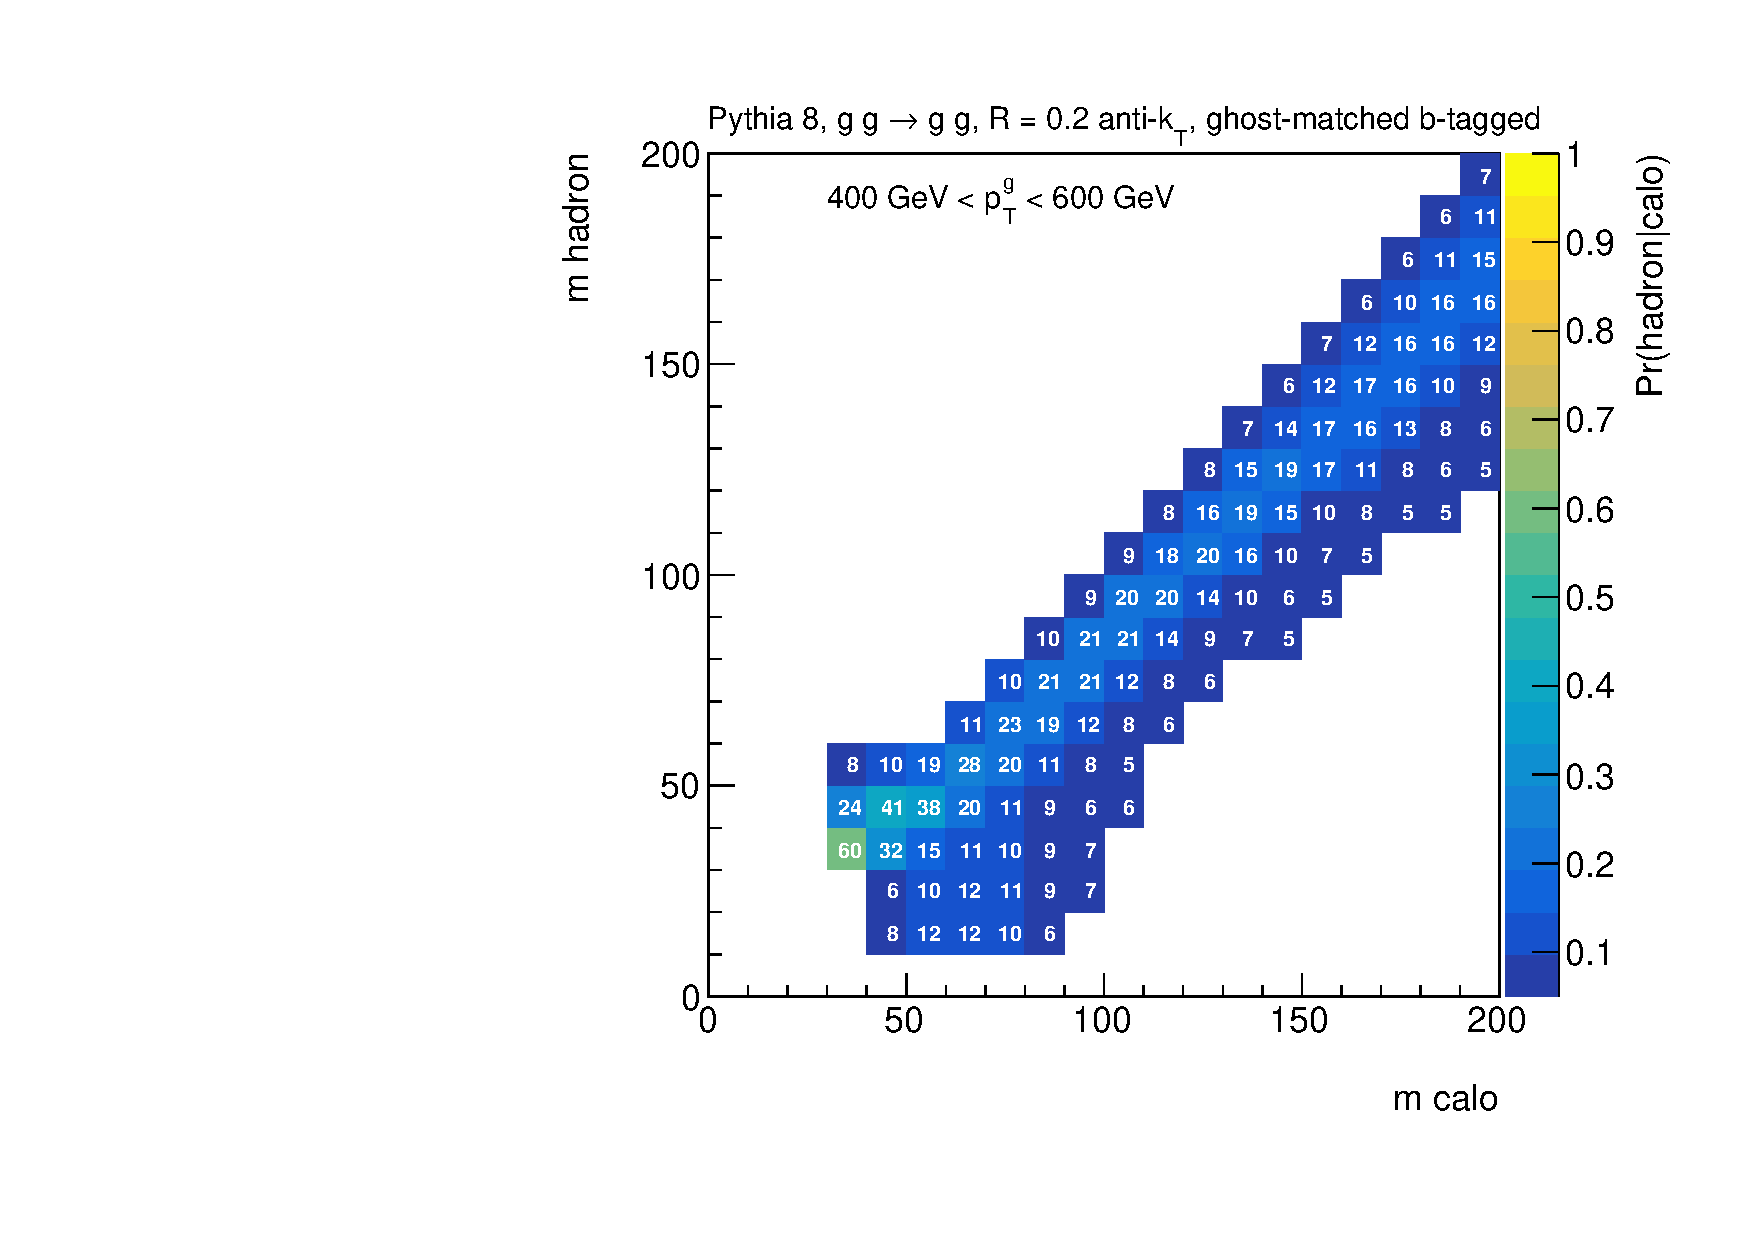
\includegraphics[width=0.45\linewidth]{figures/truth_level/m_calo_track_b}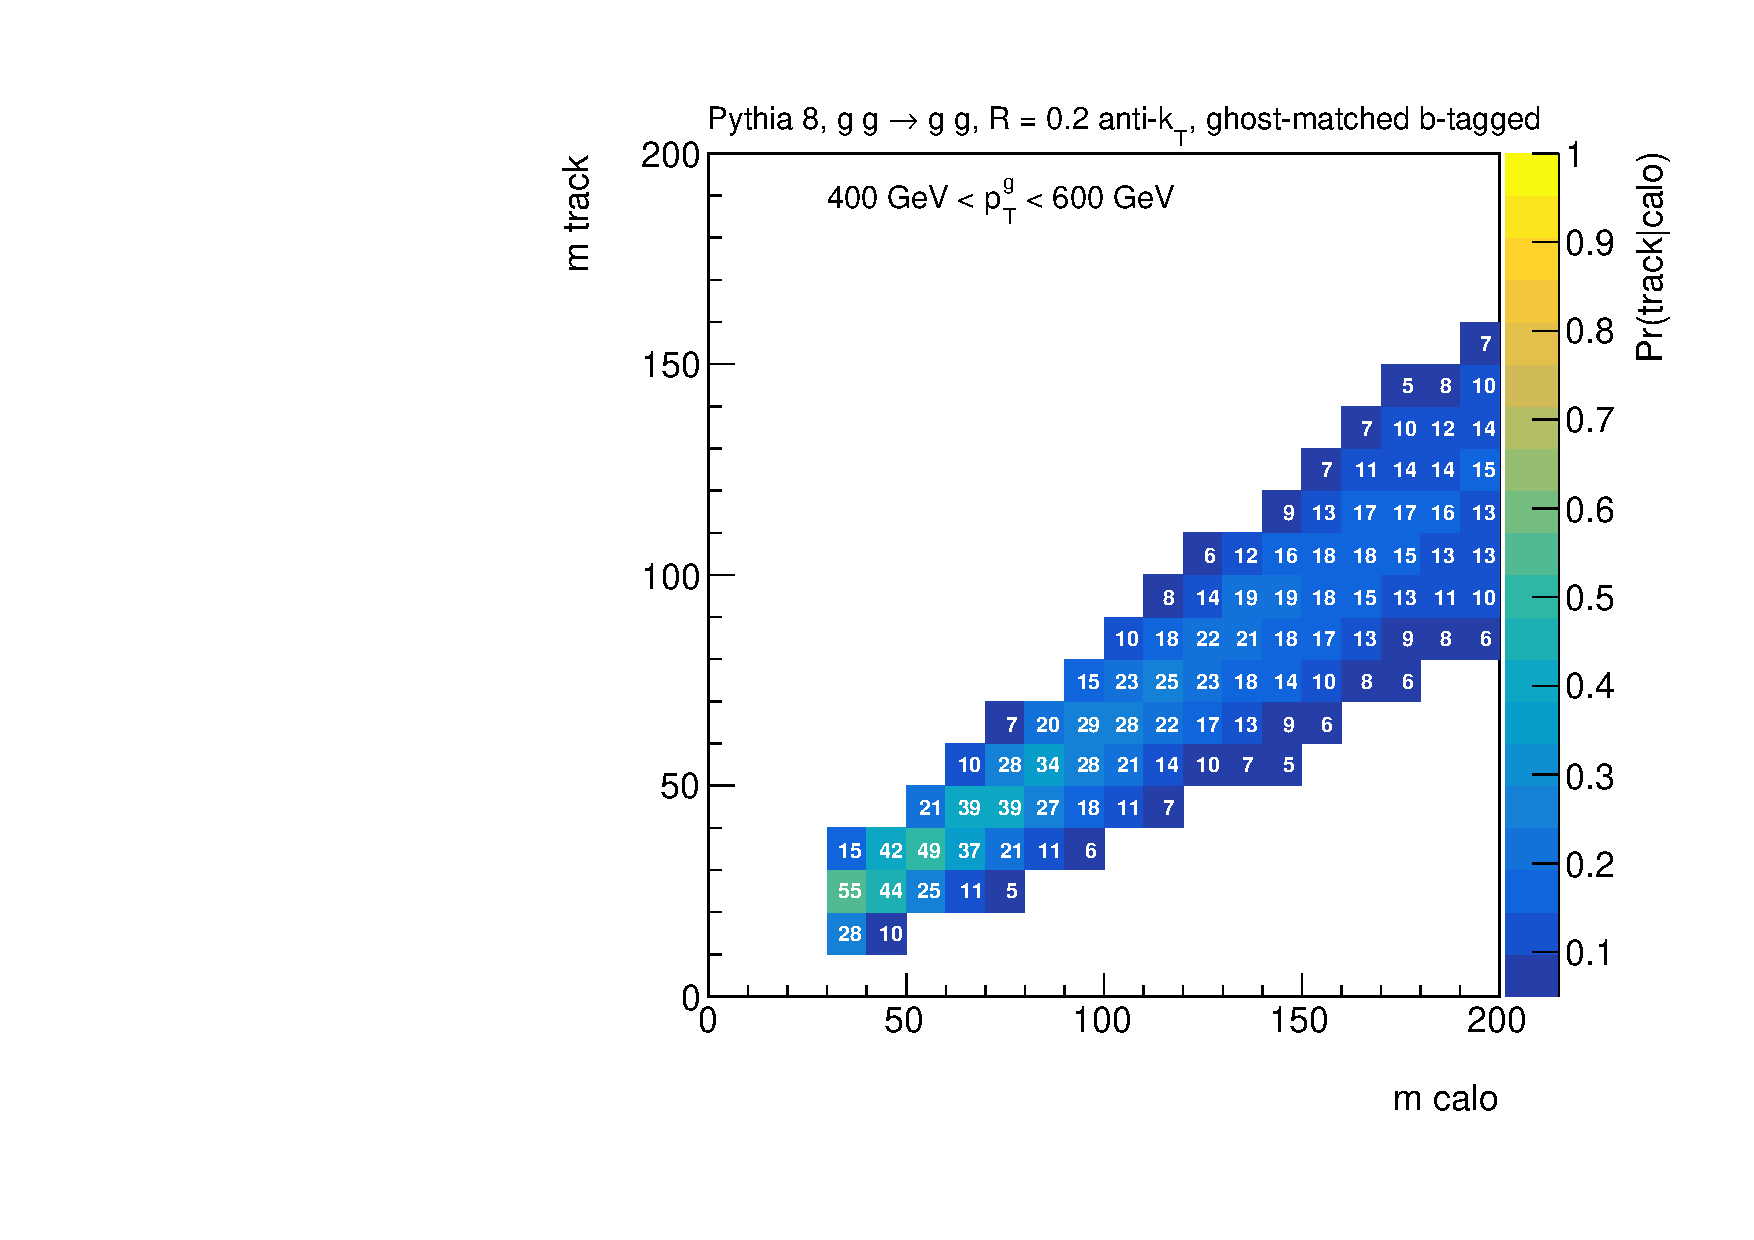
\includegraphics[width=0.45\linewidth]{figures/truth_level/m_calo_track}
\caption[]{The two-dimensional distribution of mass, but using different definitions of `b' ($B$-hadrons, $b$-jets, $b$-track-jets).} 
\label{fig:gbbresponsemass}
\end{center}
\end{figure}


\begin{figure}[htbp]
  \centering
 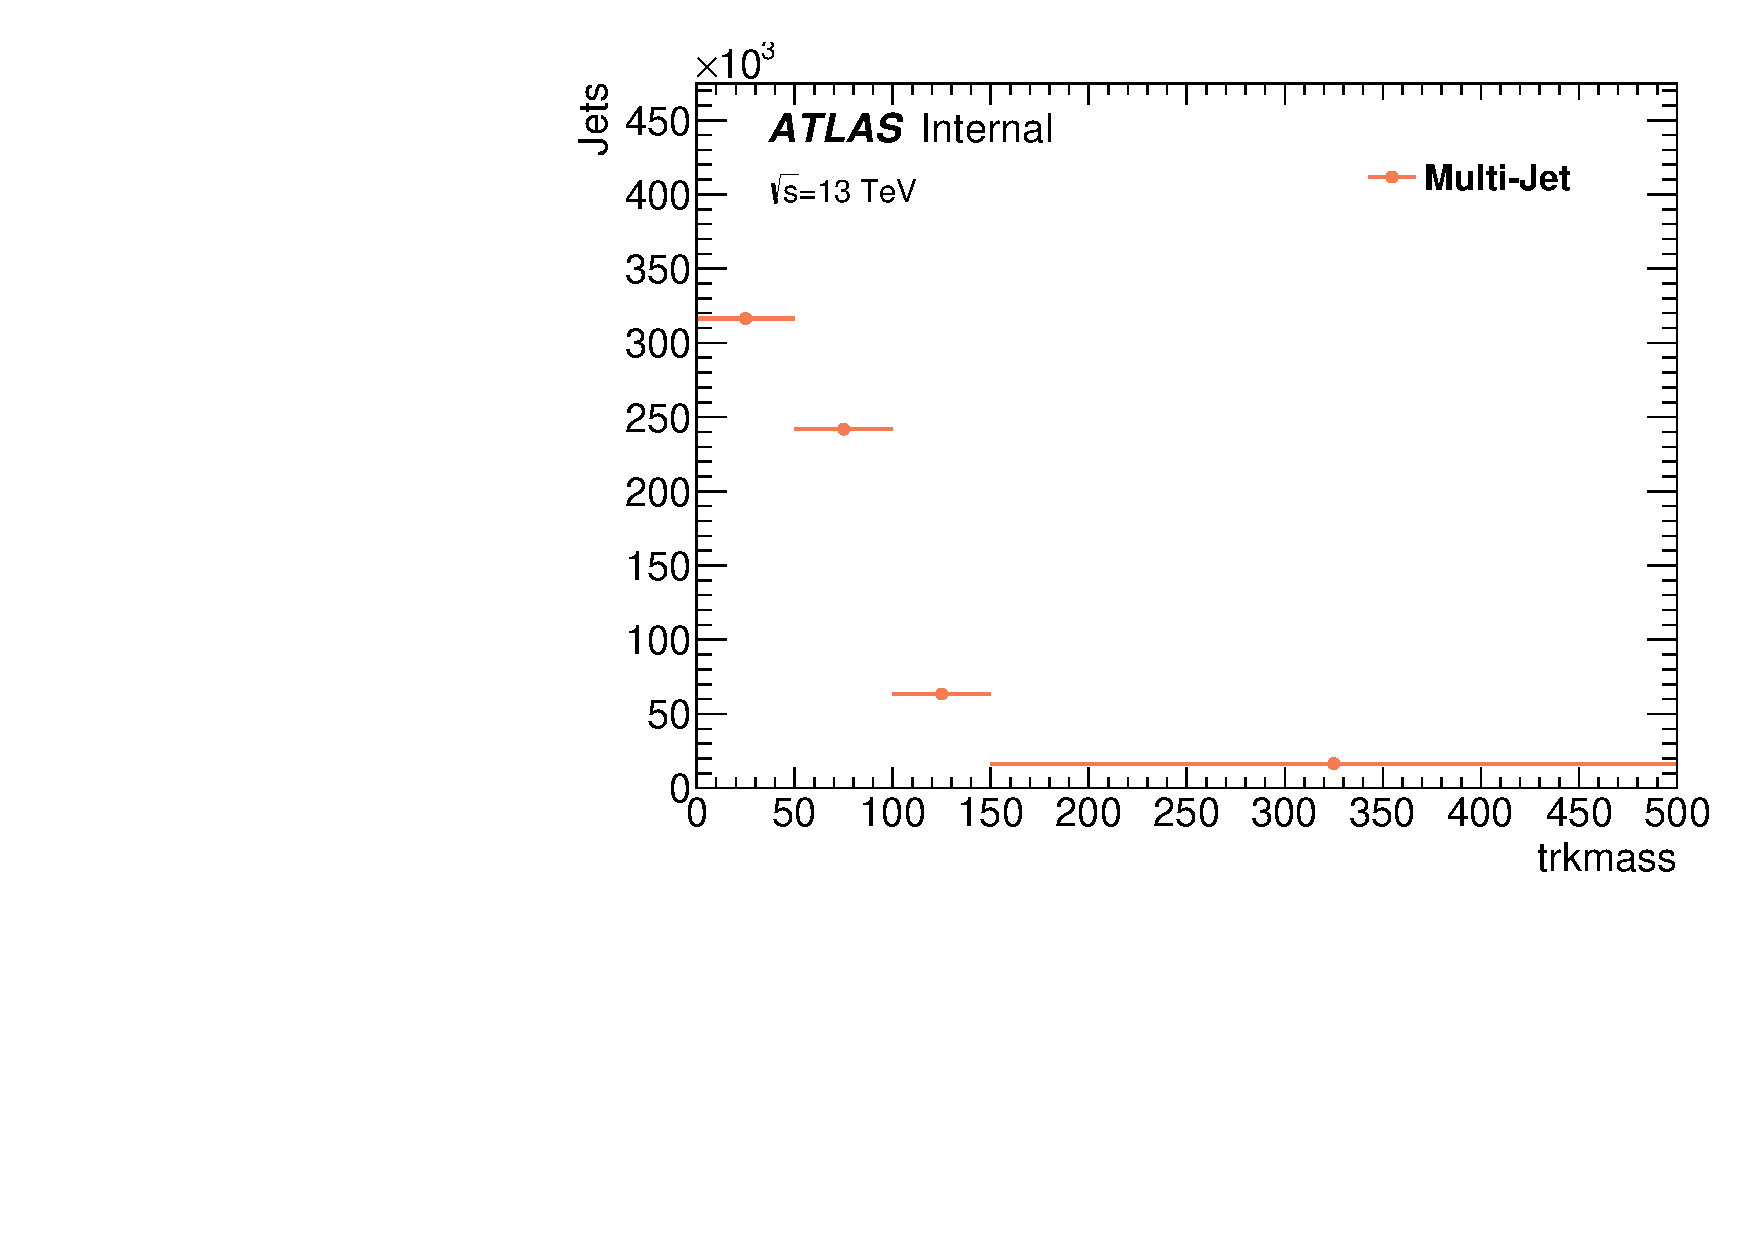
\includegraphics[width=0.6\textwidth]{figures/Sub_Sd0_Fits/Canv_trkmass_Truth.pdf}
\caption{ MC predicted distribution of $m_{b\bar b}$ }.
  \label{fig:trkmass}
\end{figure}


\begin{figure}[htbp]
  \centering
 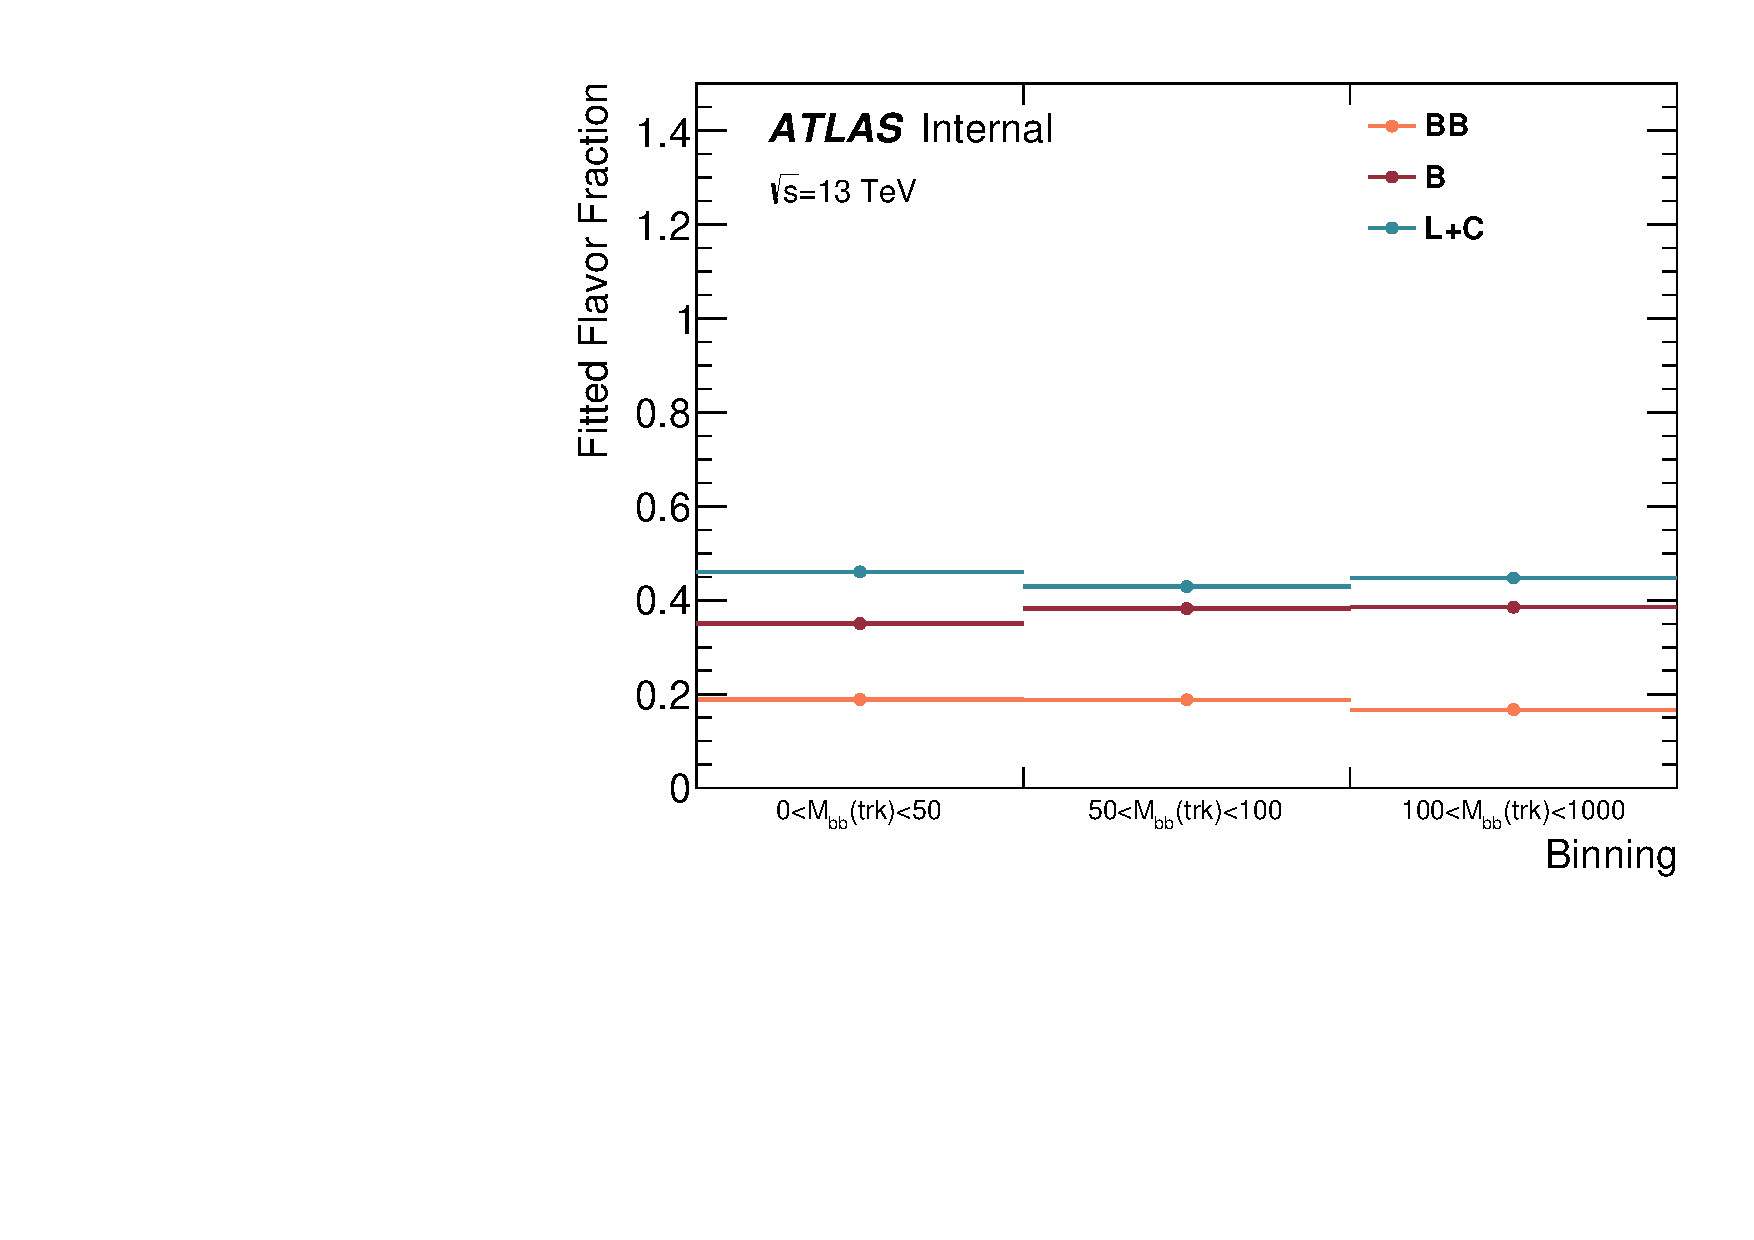
\includegraphics[width=0.45\textwidth]{figures/Sub_Sd0_Fits/Canv_trkmass_FitFrac_Original.pdf}
 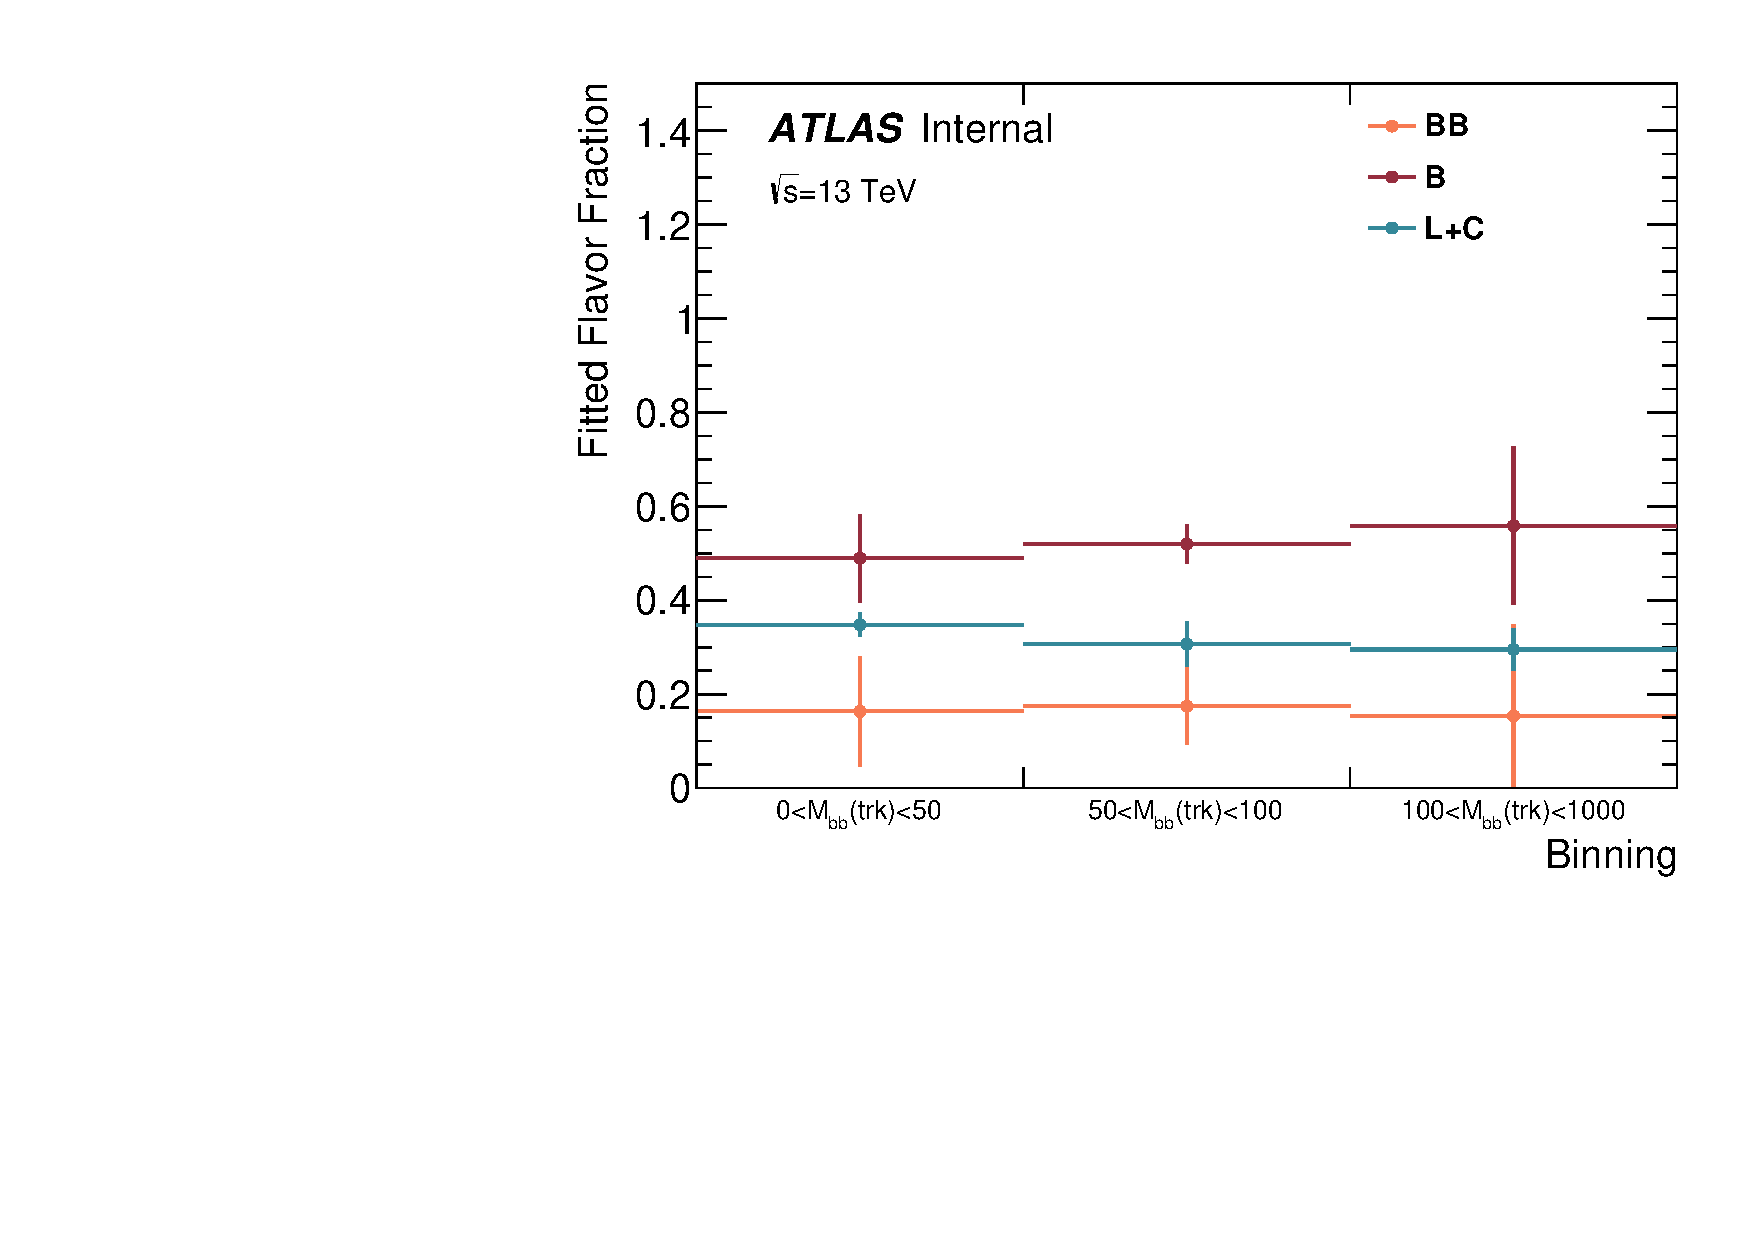
\includegraphics[width=0.45\textwidth]{figures/Sub_Sd0_Fits/Canv_trkmass_FitFrac_Corrected.pdf}

\caption{MC predicted(left) and fitted(right) flavor fraction in bins of $m_{b\bar b}$. The error bar is the quadrature sum of the uncertainty derived from fit range systematics and fit statistics as defined in Sec.\ref{sec:sub_systematics}}
  \label{fig:trkmass-fitfrac}
\end{figure}

